
\chapter{Metodologia}
\label{chap:metodologia}

\section{Tecnologias e Ferramentas Utilizadas}

A linguagem utilizada para este trabalho foi a \textit{JavaScript}, usando os recursos do \textit{Node.js}, já que foram executados longos \textit{loops} para simular milhares de mãos de \textit{Texas Hold'Em}. Tendo em vista que a quantidade de iterações poderia gerar travamentos na execução, as funções assíncronas do \textit{Node.js} \textit{(await/assync)} tornavam a execução do programa mais eficiente.

Para desenvolvimento da Rede Neural, foi utilizado o \textit{TensorFlow.js}, dispensando a necessidade de fazer uma conexão entre \textit{JavaScript} e \textit{Python} caso fosse usado apenas o \textit{TensorFlow} tradicional, sendo utilizado como referenciado por \citeonline{smilkov2019tensorflow}. Tendo em vista que o \textit{TensorFlow.js} tem funções nativas de \gls{DQN}, a mesma foi a mais adequada para o trabalho.

A plotação gráfica foi feita utilizando do \textit{Chart-Js-Node-Canvas}, \gls{API} que permite a criação dos gráficos, sendo utilizada para plotar o desempenho do agente, levando como parâmetro o ganho/perda de fichas, também representando a queda do $\epsilon$.

\section{Arquitetura do ambiente e motor de regras}

\subsection{Estrutura \texorpdfstring{\gls{MVC}}{MVC}}
Este trabalho é todo arquitetado utilizando o padrão de arquitetura \gls{MVC}, como é possível verificar no repositório de \citeonline{grangeiro2026poker}. A pasta \textit{Models} comporta as classes referentes ao \textit{Texas Hold'Em}, sendo elas a classe ``carta'' que representa as cartas do baralho utilizadas no pôquer, contendo o Naipe e o Valor da carta, e a classe ``jogador'' representa o agente, que contém as cartas disponíveis para o jogador, seu \textit{Stack} e a ação que o jogador vai tomar.
A pasta \textit{controllers} possui o controlador responsável por gerenciar as fases de apostas, sendo elas as descritas no código como:
\begin{lstlisting}[language=JavaScript, caption={Fases gerenciadas pelo jogoController.js}, label={cod:fases}]
const fases = [
        { nome: "Pre-Flop", cartas: 0 },
        { nome: "Flop", cartas: 3 },
        { nome: "Turn", cartas: 1 },
        { nome: "River", cartas: 1 }
    ];
\end{lstlisting}
A pasta \textit{Services} vai conter toda a parte estatística e da inteligência do agente, podendo ser considerada o cerébro das atividades do projeto, contendo todas as funções referentes ao baralho, a Inteligencia Artificial, os gráficos, as combinações e as estatísticas geradas pelo \textit{Monte Carlo}.
Por fim, a pasta \textit{Views} gerencia aquilo referente ao que o usuário vê durante o processamento do programa, no caso deste trabalho, controla a barra de carregamento que pode ser vista no terminal de comandos, além como as funções responsáveis por escrever informações em um arquivo de texto e uma função responsável por escrever as cartas de maneira mais compreensível para o usuário.

\subsection{Motor de avaliação - Base 15}

Um dos principais desafios para se modular as regras do pôquer são a valorização das jogadas, porém é possível superar esse desafio usando lógica simples, dando valores de força para as jogadas, entretanto cai-se em outra barreira, os empates são ocasiões incomuns, mas que são um grande desafio de serem resolvidos usando uma simples lógica de valores para as jogadas. Mesmo que o pôquer disponha do \textit{Kicker}, sendo necessário verificar qual categoria se sobressai, para seres humanos é fácil distinguir quais pares são maiores que outros, por exemplo, mas para o computadores, se o par tem sempre peso 2, independete do valor dos pares, eles serão iguais.

Para contornar isso, foi elaborado um sistema de \textit{score}(pontuação) de base 15, tomando o Ás como valor 14, a base 15 supre todas as necessidades do sistema, garantindo que não haverão possibilidades maiores que o ás, para calcular esse \textit{score} é usada a seguinte formula:

$\text{Score} = (\text{Categoria} \cdot 15^5) + \sum_{i=1}^{5} \left( \text{Carta}_i \cdot 15^{5-i} \right)$

Esta fórmula calcula o score multiplicando o valor da categoria da jogado por $15^5$, sucedido pela soma das 5(cinco) cartas que o jogador tem à sua disposição, cada uma multiplicada por uma exponenciação de base 15(quinze).
A função do código que faz esse cálculo se encontra no \textit{combinacaoService.js}, cuja é:

\newpage
\begin{lstlisting} [language=JavaScript, caption={Função de cálculo do Score}, label={cod:score}]
    const calcularScore=(categoria, v1=0, v2=0,v3=0, v4=0,
v5=0)= >{
        return categoria*759375 + v1*50625 + v2*3375 + v3*225
        + v4*15 + v5 ;
    };
\end{lstlisting}

Para melhor compreensão do motor base 15 e de como ele é utilizado de forma real no código, segue o exemplo de cálculo para a categoria \textit{Dois Pares}:

\begin{lstlisting} [language=JavaScript, caption={Função de score de Dois Pares}, label={cod:doispares}]
     if(pares.length>=2) {
        let k=kickers([pares[0], pares[1]]);
        return calcularScore(3, pares[0], pares[0], pares[1], pares[1], k[0]);
    }
\end{lstlisting}

Nesse caso, o primeiro paramêtro da função \textit{calcularscore} se refere a força da categoria, no caso de Dois pares a força é 3(três), seguido pelo par maior duas vezes como pode ser notado em \textit{pares[0], pares[0]} para ocupar os multiplicadores mais fortes, sendo esses $15^4$ e $15^3$, seguido pelos dois pares menores, que consequentemente recebem os multiplicadores mais fracos, e por fim o \textit{Kicker}, que consiste nas cartas de desempate, nesse caso sendo a última carta disponivel do agente.

Sendo assim, na rara ocasião que dois jogadores possuam Dois Pares cada um e o mesmo \textit{Kicker}, o programa é capaz de definir o que se sobressai, dando a vitória para o jogador com a maior jogada.

\section{Modelagem do agente inteligente (\textit{DQN})}

\subsection{Arquitetura e espaço de estados}

Tendo em vista que o \textit{TensorFlow.js} foi a \gls{API} selecionada para este trabalho, o mesmo foi arquitetado com duas camadas ocultas de 16 neurônios, tal quantidade foi escolhida por meio de tentativa e erro, menos neurônios deixavam o agente impreciso, mais deixavam a execução mais lenta, sem mudar significativamente os resultados, com ativação \gls{ReLU}, que cortam quaisquer números negativos que possam entrar na rede, além de uma camada de saída com 5 neurônios de ativação linear, já que o \textit{Q-Learning} retorna um score absoluto, ao invés de uma probabilidade, tudo isso pode ser denotado no seguinte trecho do código:

\begin{lstlisting}[language=JavaScript, caption={Camadas do modelo}, label={cod:camadas}]
    createModel(){
        const model=tf.sequential();
        model.add(tf.layers.dense({units: 16, inputShape: [4], activation: 'relu'}));
        model.add(tf.layers.dense({units: 16, activation: 'relu'}));
        model.add(tf.layers.dense({units: 5, activation: 'linear'}));
        model.compile({optimizer: 'adam', loss: 'meanSquaredError'});
        return model;
    }
\end{lstlisting}

Além disso, o estado do agente é composto por 4(quatro) parâmetros, sendo eles o \textit{equityMC}, que é o valor de equidade retornado pelo \textit{Monte Carlo}, o \textit{pote}, que consiste na quantidade de fichas já apostadas na rodada, a \textit{apostaParaCobrir} que representa quanto o agente deve pagar para continuar na rodada, por fim, o parâmetro \textit{minhasFichas} que diz quantas fichas disponíveis o jogador tem. Entretanto, o valor da equidade se encontra entre 0 e 1, enquanto os parâmetros baseados em fichas podem variar de 0 até 1000, sendo necessária uma normalização desses parâmetros, para não haverem conflitos no processamento do estado, é possível ver os parâmetros e a normalização no trecho a seguir:

\begin{lstlisting}[language=JavaScript, caption={Estado do jogador}, label={cod:estado}]
    obterEstado(equityMC, pote, apostaParaCobrir, minhasFichas){
        // Normalizacao basica para ajudar a rede
        return [equityMC, pote/1000, apostaParaCobrir/1000, minhasFichas/1000];
    }
\end{lstlisting}

\subsection{Espaço de ações}

Considerando que as apostas no \textit{Texas Hold'Em} são o fator mais importante para o jogo, é extremamente importante que o agente consiga executa-las de maneira consistente, entretanto, como no jogo tradicional as apostas tem valores extremamente imprecisos, podendo variar entre 1 até o todas as fichas disponíveis do jogador, e isso se tornaria um empecilho para o \textit{Q-Learning}, sendo assim, foi feita uma discretização das ações.

Como citado anteriormente, a rede neural possui 5 neurônios de saída, que podem ser ditos como as ações que o agente toma, sendo eles os seguintes:
\begin{itemize}
    \item \textit{Fold}: O agente desiste da mão;
    \item \textit{Check/call}: O agente paga as apostas que vem na mesa, ou passa a vez caso não tenham apostas à serem pagas;
    \item \textit{Raise Leve}: O agente adiciona mais 150 fichas na aposta que vem para ele pagar;
    \item \textit{Raise Forte}: O agente adiciona mais 300 fichas na aposta que vem para ele pagar;
    \item \textit{All In}: O agente aposta todas as suas fichas disponíveis.
\end{itemize}

\subsection{Modelagem das recompensas}

As recompensas são a principal forma de se treinar um agente por reforço. Seguindo as regras do \textit{Texas Hold'Em}, as recompensas podem ser dadas simplesmente pelo lucro ou prejuízo de fichas, entretanto apenas usar o lucro/prejuízo do agente pode encaminha-lo para ótimos locais, como dito por \citeonline{russell2010artificial}, um ótimo local é quando o agente ``descobre'' a melhor forma para o que ele aprendeu, mesmo que fuja do ótimo global, que seria a tomada de decisão ideal, no caso deste trabalho, o agente atingiu um ótimo local em que o mesmo sempre desistia de todas as mãos, assim ele não perdia fichas. Para contornar isso, foi utilizada a estratégia de \textit{Blinds}, que são apostas rotativas no \textit{Texas Hold'Em} que forçam o agente a apostar na primeira rodada, o que resolveu o ótimo local do \text{fold} na primeira fase, porém, o agente aprendeu que caso apenas desse \textit{Check}, também perderia o mínimo de fichas possiveis. Sendo assim, foi necessário a implementação de uma penalização por passividade, associado de uma bonificação por agressividade, como denonado por \citeonline{ng1999policy}, sendo feita como indicado na Figura 2:

\begin{figure}[htbp]
    \centering
    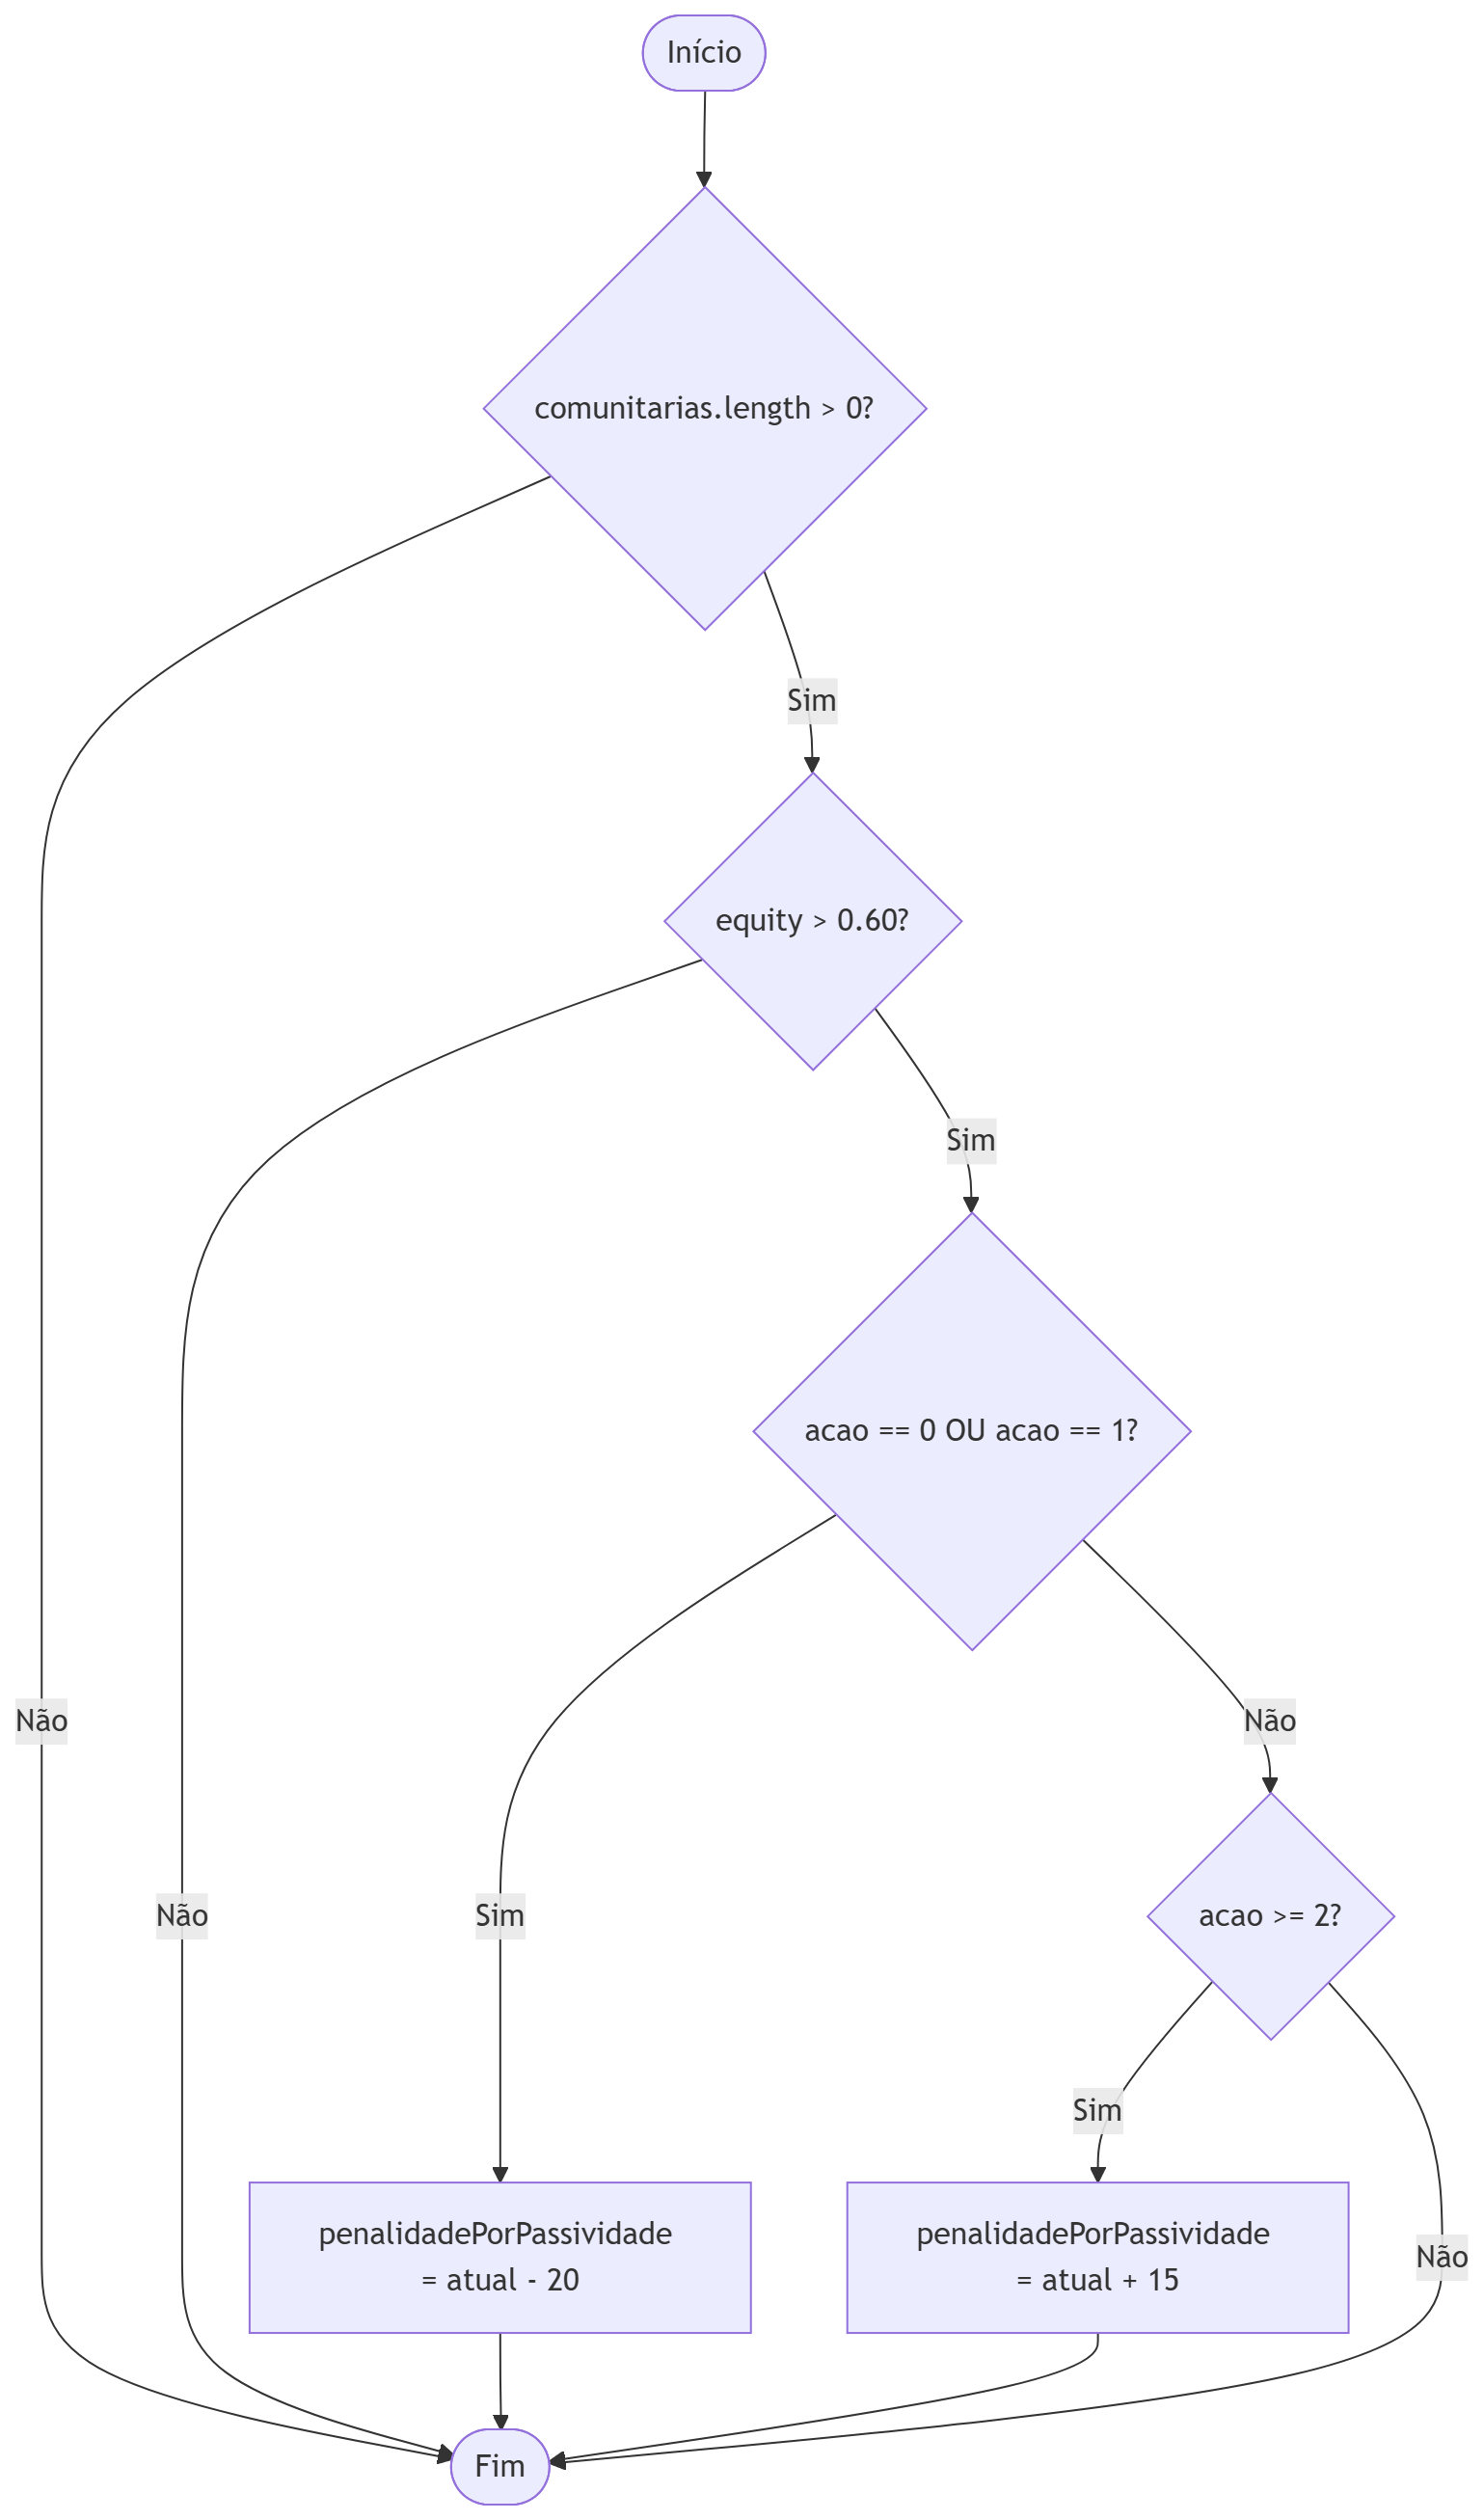
\includegraphics[width=0.5\linewidth]{lib/Fluxograma das penalidades.png}
    \caption{Fluxograma do sistema de penalidade por passividade: Autoria própria}
    \label{fig:desempenhoAgente}
\end{figure}

Como pode ser visto, caso o agente tenha um \textit{equity} superior a 60\%, o mesmo é penalizado em 20 pontos caso escolha a ação de \textit{Fold} ou de \textit{Check}, enquanto recebe uma bonificação de mais 15 quando faz uma jogada agressiva, como aumentar a aposta ou até mesmo dar \textit{all-in}.
Sendo assim, o agente evita os ótimos locais mencionados, além de deixar o sistema de recompensas mais robusto, fazendo que o agente seja mais assertivo conforme aprende a jogar o jogo

\section{Cenários de simulação e Treinamento}

\subsection{O ambiente da mesa}

O ambiente foi configurado para comportar 4 agentes que fazem o papel de jogador, cada um iniciando com um \textit{Stack efetivo}(fichas inicias) de 1000 fichas, com a existência do \textit{Small Blind} e do \textit{Big Blind}, sendo apostas obrigatórias rotativas que os jogadores são obrigados a pagar quando são selecionados, cobrindo todos os jogadores da mesa.

\subsection{A execução dos treinos}

O treinamento ocorre por grandes lotes contínuos de partidas, com exemplo de 10.000 mãos sendo feitas, cada mão podendo ser repetida pela \gls{RNA}, usando assim uma simulação em vários cenários, como descrito por \citeonline{leonelli2021montecarlo}, aplicando os \textit{Experience Replay} utilizando lotes de 32 memórias no final de todas as mãos.

\subsection{O decaimento do \textit{Epsilon}}

Sendo usado como fator de aleatoriedade nas primeiras mãos, já que o agente não sabe como jogar no inicio, o $\epsilon$ é iniciado em 1.0, definindo aleatoriedade total no começo das simulações, decaindo em 0.5\% a cada mão, chegando até o valor mínimo de 0.01 , esse decaimento é definido no seguinte trecho de código:

\begin{lstlisting}[language=JavaScript, caption={Variáveis responsáveis pelo controle do epsilon}, label={cod:varEpsilom}]
        this.epsilon=1.0;
        this.epsilonMin=0.01; 
        this.epsilonDecay=0.995; 
\end{lstlisting}

Tendo isso em vista, o $\epsilon$ é decrementado no fim de cada simulação da seguinte maneira:

\begin{lstlisting}[language=JavaScript, caption={Decaimento do epsilon}, label={cod:decaEpsilom}]
        if(this.epsilon>this.epsilonMin){
            this.epsilon*=this.epsilonDecay;
        }
\end{lstlisting}
